%%%%%%%%%%%%%%%%%%%%%%%%%%%%%%%%%%%%%%%%%
% Lachaise Assignment
% LaTeX Template
% Version 1.0 (26/6/2018)
%
% This template originates from:
% http://www.LaTeXTemplates.com
%
% Authors:
% Marion Lachaise & François Févotte
% Vel (vel@LaTeXTemplates.com)
%
% License:
% CC BY-NC-SA 3.0 (http://creativecommons.org/licenses/by-nc-sa/3.0/)
%
%%%%%%%%%%%%%%%%%%%%%%%%%%%%%%%%%%%%%%%%%

%----------------------------------------------------------------------------------------
%	PACKAGES AND OTHER DOCUMENT CONFIGURATIONS
%----------------------------------------------------------------------------------------

\RequirePackage[hyphens]{url}

\documentclass{article}

\usepackage{dirtree}
\usepackage{hyperref}
%\PassOptionsToPackage{hyphens}{hyperref}

%%%%%%%%%%%%%%%%%%%%%%%%%%%%%%%%%%%%%%%%%
% Lachaise Assignment
% Structure Specification File
% Version 1.0 (26/6/2018)
%
% This template originates from:
% http://www.LaTeXTemplates.com
%
% Authors:
% Marion Lachaise & François Févotte
% Vel (vel@LaTeXTemplates.com)
%
% License:
% CC BY-NC-SA 3.0 (http://creativecommons.org/licenses/by-nc-sa/3.0/)
% 
%%%%%%%%%%%%%%%%%%%%%%%%%%%%%%%%%%%%%%%%%

%----------------------------------------------------------------------------------------
%	PACKAGES AND OTHER DOCUMENT CONFIGURATIONS
%----------------------------------------------------------------------------------------

\usepackage{amsmath,amsfonts,stmaryrd,amssymb} % Math packages

\usepackage{enumerate} % Custom item numbers for enumerations

\usepackage[ruled]{algorithm2e} % Algorithms

\usepackage[framemethod=tikz]{mdframed} % Allows defining custom boxed/framed environments

\usepackage{listings} % File listings, with syntax highlighting
\lstset{
	basicstyle=\ttfamily, % Typeset listings in monospace font
}

%----------------------------------------------------------------------------------------
%	DOCUMENT MARGINS
%----------------------------------------------------------------------------------------

\usepackage{geometry} % Required for adjusting page dimensions and margins

\geometry{
	paper=a4paper, % Paper size, change to letterpaper for US letter size
	top=2.5cm, % Top margin
	bottom=3cm, % Bottom margin
	left=2.5cm, % Left margin
	right=2.5cm, % Right margin
	headheight=14pt, % Header height
	footskip=1.5cm, % Space from the bottom margin to the baseline of the footer
	headsep=1.2cm, % Space from the top margin to the baseline of the header
	%showframe, % Uncomment to show how the type block is set on the page
}

%----------------------------------------------------------------------------------------
%	FONTS
%----------------------------------------------------------------------------------------

\usepackage[utf8]{inputenc} % Required for inputting international characters
\usepackage[T1]{fontenc} % Output font encoding for international characters

\usepackage{XCharter} % Use the XCharter fonts

%----------------------------------------------------------------------------------------
%	COMMAND LINE ENVIRONMENT
%----------------------------------------------------------------------------------------

% Usage:
% \begin{commandline}
%	\begin{verbatim}
%		$ ls
%		
%		Applications	Desktop	...
%	\end{verbatim}
% \end{commandline}

\mdfdefinestyle{commandline}{
	leftmargin=10pt,
	rightmargin=10pt,
	innerleftmargin=15pt,
	middlelinecolor=black!50!white,
	middlelinewidth=2pt,
	frametitlerule=false,
	backgroundcolor=black!5!white,
	frametitle={Command Line},
	frametitlefont={\normalfont\sffamily\color{white}\hspace{-1em}},
	frametitlebackgroundcolor=black!50!white,
	nobreak,
}

% Define a custom environment for command-line snapshots
\newenvironment{commandline}{
	\medskip
	\begin{mdframed}[style=commandline]
}{
	\end{mdframed}
	\medskip
}

%----------------------------------------------------------------------------------------
%	FILE CONTENTS ENVIRONMENT
%----------------------------------------------------------------------------------------

% Usage:
% \begin{file}[optional filename, defaults to "File"]
%	File contents, for example, with a listings environment
% \end{file}

\mdfdefinestyle{file}{
	innertopmargin=1.6\baselineskip,
	innerbottommargin=0.8\baselineskip,
	topline=false, bottomline=false,
	leftline=false, rightline=false,
	leftmargin=2cm,
	rightmargin=2cm,
	singleextra={%
		\draw[fill=black!10!white](P)++(0,-1.2em)rectangle(P-|O);
		\node[anchor=north west]
		at(P-|O){\ttfamily\mdfilename};
		%
		\def\l{3em}
		\draw(O-|P)++(-\l,0)--++(\l,\l)--(P)--(P-|O)--(O)--cycle;
		\draw(O-|P)++(-\l,0)--++(0,\l)--++(\l,0);
	},
	nobreak,
}

% Define a custom environment for file contents
\newenvironment{file}[1][File]{ % Set the default filename to "File"
	\medskip
	\newcommand{\mdfilename}{#1}
	\begin{mdframed}[style=file]
}{
	\end{mdframed}
	\medskip
}

%----------------------------------------------------------------------------------------
%	NUMBERED QUESTIONS ENVIRONMENT
%----------------------------------------------------------------------------------------

% Usage:
% \begin{question}[optional title]
%	Question contents
% \end{question}

\mdfdefinestyle{question}{
	innertopmargin=1.2\baselineskip,
	innerbottommargin=0.8\baselineskip,
	roundcorner=5pt,
	nobreak,
	singleextra={%
		\draw(P-|O)node[xshift=1em,anchor=west,fill=white,draw,rounded corners=5pt]{%
		Question \theQuestion\questionTitle};
	},
}

\newcounter{Question} % Stores the current question number that gets iterated with each new question

% Define a custom environment for numbered questions
\newenvironment{question}[1][\unskip]{
	\bigskip
	\stepcounter{Question}
	\newcommand{\questionTitle}{~#1}
	\begin{mdframed}[style=question]
}{
	\end{mdframed}
	\medskip
}

%----------------------------------------------------------------------------------------
%	WARNING TEXT ENVIRONMENT
%----------------------------------------------------------------------------------------

% Usage:
% \begin{warn}[optional title, defaults to "Warning:"]
%	Contents
% \end{warn}

\mdfdefinestyle{warning}{
	topline=false, bottomline=false,
	leftline=false, rightline=false,
	nobreak,
	singleextra={%
		\draw(P-|O)++(-0.5em,0)node(tmp1){};
		\draw(P-|O)++(0.5em,0)node(tmp2){};
		\fill[black,rotate around={45:(P-|O)}](tmp1)rectangle(tmp2);
		\node at(P-|O){\color{white}\scriptsize\bf !};
		\draw[very thick](P-|O)++(0,-1em)--(O);%--(O-|P);
	}
}

% Define a custom environment for warning text
\newenvironment{warn}[1][Warning:]{ % Set the default warning to "Warning:"
	\medskip
	\begin{mdframed}[style=warning]
		\noindent{\textbf{#1}}
}{
	\end{mdframed}
}

%----------------------------------------------------------------------------------------
%	INFORMATION ENVIRONMENT
%----------------------------------------------------------------------------------------

% Usage:
% \begin{info}[optional title, defaults to "Info:"]
% 	contents
% 	\end{info}

\mdfdefinestyle{info}{%
	topline=false, bottomline=false,
	leftline=false, rightline=false,
	nobreak,
	singleextra={%
		\fill[black](P-|O)circle[radius=0.4em];
		\node at(P-|O){\color{white}\scriptsize\bf i};
		\draw[very thick](P-|O)++(0,-0.8em)--(O);%--(O-|P);
	}
}

% Define a custom environment for information
\newenvironment{info}[1][Info:]{ % Set the default title to "Info:"
	\medskip
	\begin{mdframed}[style=info]
		\noindent{\textbf{#1}}
}{
	\end{mdframed}
}
 % Include the file specifying the document structure and custom commands

%----------------------------------------------------------------------------------------
%	ASSIGNMENT INFORMATION
%----------------------------------------------------------------------------------------

\title{\textbf{"CAESAR SAID WHAT?!":\\ Breaking Substitution Ciphers Programatically}} % Title of the assignment

%\author{Yukiko Amagi\\ \texttt{y.amagi@inabauniversity.jp}} % Author name and email address

\date{} % University, school and/or department name(s) and a date

%----------------------------------------------------------------------------------------

\begin{document}

\maketitle % Print the title

%----------------------------------------------------------------------------------------
%	INTRODUCTION
%----------------------------------------------------------------------------------------

\section*{Introduction}

One of the most basic and oldest forms of encryption is the substitution cipher. The substitution cipher is a simple encryption technique where every character of some text, known as the \textbf{plaintext}, is encrypted by replacing every letter with another letter, forming encrypted text, known as a \textbf{ciphertext}. Using substitution ciphers is simple and easy to use but unfortunately it is not secure enough to hold up to more advanced cryptanalysis.

In this project we will be exploring two simple substitution ciphers: The Caesar Cipher and an arbitrary Monoalphabeteic Cipher. We'll get a good understanding of each cipher and create programs that could automate the cracking of such simple ciphers. At the same time we'll also exercise our ability to manipulate strings and parse files within program languages.

\section{The Caesar cipher}
Let's start off by taking a look at the Caesar Cipher. A Caesar Cipher is a simple cipher where each letter within some plaintext is replaced by a letter at some fixed offset down the alphabet. For example, if you were to use a Caesar Cipher with an offset of +4, the letter "A" would be replaced with the letter "E" since "E" is +4 positions after "A". Figure 1 shows the resulting alphabet mapping resulting from a Caesar Cipher with the offset +4.\\


\begin{figure}[h!]
 \centering
  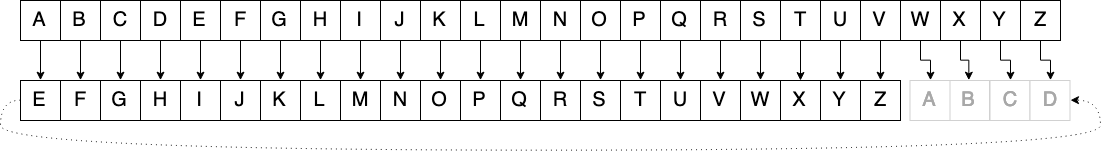
\includegraphics[width=1\textwidth]{caesarcipher}
 \caption{Example of Caesar Cipher with an offset of +4}
 \end{figure}

You can think of the Caesar Cipher as mapping letters based on indexes. We can generalize the caesar cipher with the following equation:
Given some letter with an index of $x$, and some offset $k$, the index of the new letter $E(x)$ would be:
$$E_n(x)=(x+k)\mod 26$$

\subsection{Breaking the Caesar Cipher}
\subsubsection*{Exploiting the limitations of the Caesar Cipher for a Brute Force Attack}
We know that the Caesar Cipher simply offsets the original alphabet by some value, so the number of ways of encrypting a message with a caesar would be equal to the amount of ways you can offset the original alphabet. If you notice, starting from offset 0 (which is the original alphabet), you can offset the alphabet 25 times before you return to the original alphabet.

Since we know that there are only 25 ways to possibly offset an alphabet within a Caesar Cipher, we can feasibly brute force the decryption of a ciphertext decrypted with a Caesar Cipher by generating all possible plaintexts at each offset and picking the one that makes the most sense.

\subsubsection*{Determining the correct plaintext}
When using brute force to generate possible decrypted plaintexts, It is easy for a human to determine which plaintext is the correct plaintext as we know what the English language "should" look like. However that is not good enough as we are trying to break the caesar cipher in a completely programmatic way. How can we let computer program figure out which plaintext is correct and makes sense?

A simple and naive way to go about it is to have the computer program check the words of a plaintext against a dictionary/list of actual English words to determine which words "makes sense". This way, a program can determine which decrypted plaintext is most likely the correct plaintext by finding the plaintext with the most amount of words that "make sense".

\subsection{Program Implementation}
For this part of the assignment you will be creating a program called CrackCaesar that will decrypt a ciphertext using brute force and a dictionary of common words. \\

\noindent In general, your CrackCaesar program will do the following:
\begin{enumerate}
\item Take in two text files as arguments (in order):
\begin {enumerate}
	\item A text file containing ciphertext needing to be decrypted
	\item A text file containing common words to check your plaintext against
\end{enumerate}
\item Break the ciphertext using brute force, determining the correct decoded plaintext by checking if decoded words match words in the text file of common words.
\item Print out the determined offset for the Casesar Cipher and the decoded plaintext. (Note: The case of the output does not matter)
\end{enumerate}

\noindent \\You can implement your program with any of the following languages:
\begin{itemize}
\item Python
\item Java
\item C/C++
\end{itemize}
\-\\\ Under the following constraints:
\begin{itemize}
\item \textbf{The name of your implementation should be CrackCaesar exactly.} Our grading scripts will compile the program if necessary, and call the program accordingly with the proper arguments. Using your program should look along the lines of the following:
	\begin{itemize}
	\item For Python:
		\begin{verbatim}
			        $ python CrackCaesar.py ciphertext.txt dictionary.txt
		\end{verbatim}
	\item For Java:
		\begin{verbatim}
			        $ java CrackCaesar ciphertext.txt dictionary.txt
		\end{verbatim}
	\item For C/C++:
		\begin{verbatim}
			        $ ./CrackCaesar ciphertext.txt dictionary.txt
		\end{verbatim}
	\end{itemize}
\item \textbf{Keep your implementation to one file.} This requirement is for those that chose a compiled language. This will make compilation easy and straight forward.
\item \textbf{You can only use the standard libraries.} Do not use any libraries outside of the standard libraries for your programming language. This is to ensure we don't have download anything extra when grading.
\end{itemize}


\subsection{Example Run}
To show a better example imagine, we have a text within the ciphertext called $ciphertext.txt$ and our dictionary of common words called $dictionary.txt$.

% File contents
\begin{file}[ciphertext.txt]
\begin{lstlisting}[language=Python]
aopz tlzzhnl pz jvtwslalsf jvumpkluaphs.
p opk aol tvulf ha aol lknl vm aol zhohyh
klzlya
\end{lstlisting}
\end{file}

% File contents
\begin{file}[dictionary.txt]
\begin{lstlisting}[language=Python]
you
it
not
or
be
are
from
.......
\end{lstlisting}
\end{file}

Running the program written in python should look like the following:

% Command-line "screenshot"
\begin{commandline}
	\begin{verbatim}
		$ python CrackCaesar.py ciphertext.txt dictionary.txt
		7
		this message is completely confidential. i hid the money at the edge
		of the sahara desert
	\end{verbatim}
\end{commandline}

\subsection{Testing your program}
In order to test your program, provided should be a folder called \textbf{SampleCaesarTexts} with two sample text files
\begin{enumerate}
\item \textbf{ciphertext-sample.txt} - a sample ciphertext encrypted using a caesar cipher
\item \textbf{dictionary-sample.txt} - a text file containing common words separated by line
\item \textbf{plaintext-sample.txt} - the correct plaintext that your program should output
\end{enumerate}

\begin{info}[Note:] % Information block
The sample dictionary is based on 10,000 of the most common words determined by analysis of Google's Trillion Word Corpus. You can learn more here: \url{https://github.com/first20hours/google-10000-english}
\end{info}

\begin{info}[Correctness:] % Information block
The correct output of your program should when decrypting ciphtertext-sample.txt should be similar to the contents of  plaintext-sample.txt. Do not worry about the case of the letters if your program outputs different letter cases, they will be ignored. Note that the sample ciphertext is merely a sample and will not be used when testing your program so make sure you implement your program correctly!
\end{info}



\section{General Monoalphabetic Substitution Ciphers}
The caesar cipher is just a simple example of what is known as a \textbf{monoalphabetic cipher}, a cipher where each letter from the original alphabet text is encrypted using some fixed alphabet mapping. This means each letter is replaced by one other letter. In the case of the Caesar Cipher, the fixed alphabet mapping was simply the original alphabet offset by a certain value, but in general the mapping for a monoalphabetic cipher can be completely arbitrary. Notice in figure 2 and 3 how each letter is mapped to exactly 1 other letter, with no noticeable patterns within the letter assignments.\\

\begin{figure}[h!]
 \centering
  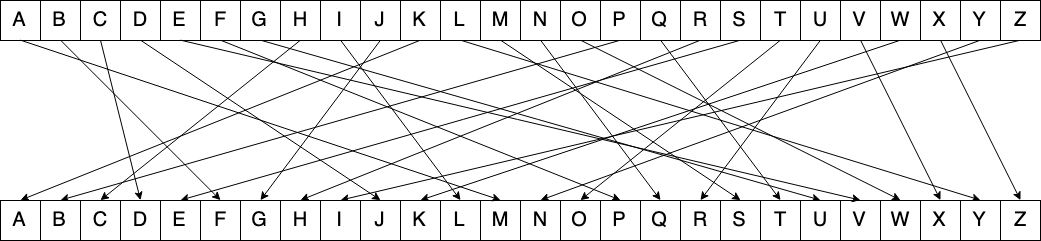
\includegraphics[width=1\textwidth]{monocipher1}
 \caption{Example of an arbitrary mapping for a monoalphabetic cipher}
 \end{figure}


 \begin{figure}[h!]
 \centering
  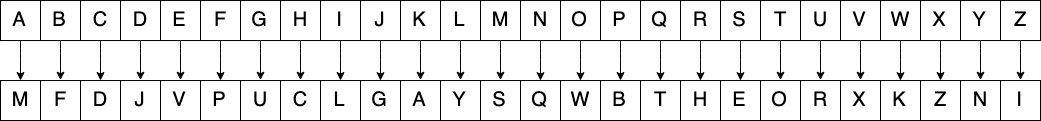
\includegraphics[width=1\textwidth]{monocipher2}
 \caption{Resulting alphabet mapping from figure 2}
 \end{figure}


\subsection{Breaking a Monoalphabetic Cipher}

\subsubsection*{Using Brute Force}
Breaking the Caesar Cipher using brute force is easy as alphabet mappings are determined by an offset making the alphabet key space to search was limited to 26 possible offsets. (or 25 if you exclude offsetting by 0). But what if the alphabet mappings were arbitrary? By this we mean, where letter assignment is not bounded by any order/offset?\\

\noindent In order to crack the an arbitrary substitution cipher using brute force we will have to try every alphabet mapping possible to decrypt every possible plaintext. Assigning a letter to letters A-Z, we would assign 26 of the possible letters to letter A, then assign one of the remaining 25 letters to B and so on. In the end we would can see that number of alphabet mappings to search is:
$$26 \times 25 \times 24 \times \cdots \times 1 = 26! = ~4.03 \times 10^{26}$$
To try out 403 septillion alphabet mappings is a lot to do, even for a computer. To put that into a more relatable perspective, 403 septillion is a bit more than the the square of 20 trillion ($20 \times 10^{12}$) and far greater than the number of sand grains on planet Earth ($7.5 \times 10^{18}$). Nonetheless, you can still try and crack an arbitrary monoalphabetic cipher using brute force, but it will take a long, long, long, time.

\subsubsection*{Frequency Analysis: A Better Approach }
A better approach to breaking a monoalphabetic substitution cipher is to use frequency analysis. \textbf{Frequency analysis} is the study of the frequency of letters or sets of letters. Like every language, the English language has rules that determine what letters we can be used together to form words. Because of these rules, the English language tends to exhibit certain characteristics in terms of letter frequency. By examining the letter frequencies, we can potentially get some idea of which letters map to which.

\begin{figure}[h!]
 \centering
  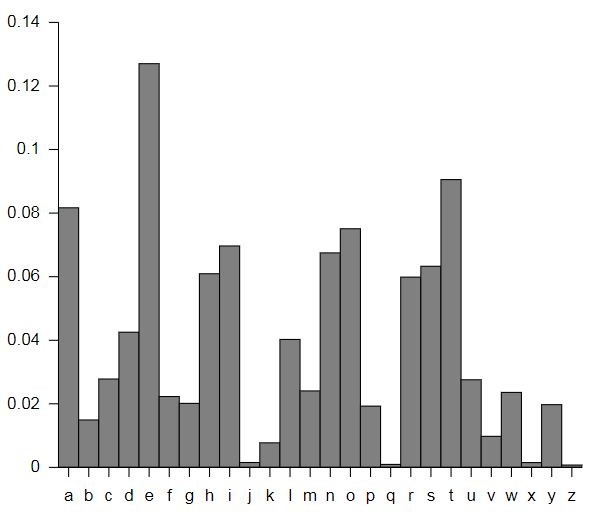
\includegraphics[width=.5\textwidth]{letterfrequency}
 \caption{Typical distribution of letters in the English language \textit{(source: wiki)}}
 \end{figure}

 \subsubsection*{Getting Accurate Statistics for Frequency Analysis}
Figure 4 shows the typical letter distribution of letters within the English language. These frequencies could be used to help decipher most ciphertexts but the use of these letter frequencies may be too general to be used for more elaborate ciphertexts. How can we get better statistical results to aid in deciphering a ciphertext in question? One approach to this problem is to perform a frequency analysis on texts that potentially relate to the ciphertext. The idea is that related texts could exhibit similar sentence structures and word use. Because of this, using related known texts could potentially give us better statistical results that could be used to decipher the ciphertext faster.

If letter frequencies from known texts don't help up give the write alphabet mapping, we can further analyze the frequencies of groups of letters called $N$-grams, which are sets of $N$ consecutive letters. $N$-grams could give a deeper insight of patterns within texts and can give more hints on possible letter mappings.


\subsection{Program Implementation}
For this part of the assignment we will only focus on individual letter frequencies. You will create a program called $CrackCipher$ that will analyze a set of known texts and decrypt a ciphertext by matching up letter frequencies. You can assume that relative letter frequencies of "known texts" will be perfectly representative of the relative letter frequencies within the ciphertext. By "perfect", we mean that matching letters based on relative letter frequencies will result in a correct alphabet mapping.\\

To make it slightly harder provided ciphertexts will also have spaces substituted.  This means the substitution cipher allows for the space character to be used to subsitute any other letter and vice versa. This is a more realistic way of using a sustitution cipher as doing this will hide the seperation between words making it impossible to deduce letter mappings based on word lengths in ciphertexts. Fortunately despite being able to hide words, it is quite easy to determine what letter maps to the space character with frequency analysis as more often than not, the space character is the most frequent character within a given text.\\

\noindent Your $CrackCipher$ program will do the following:
\begin{enumerate}
\item Take in two arguments (in order)
\begin{enumerate}
	\item A text file containing ciphertext needing to be decoded
	\item A fairly long text file containing known text related to the plaintext trying to be recovered
\end{enumerate}
\item Perform frequency analysis on the letters within the known text (including spaces).
\item Perform frequency analysis on the letters within the ciphertext (including spaces).
\item Generate an alphabet mapping to use based on similar letter frequencies (which includes mapping the space character).
\item Print out the decoded plaintext using the determined alphabet key. (Note: The case of the output does not matter)
\end{enumerate}

Note: When parsing texts, be sure not to confuse newline characters with spaces

\noindent \\ Similar to the last program, you can implement your program with any of the following languages:
\begin{itemize}
\item Python
\item Java
\item C/C++
\end{itemize}
\-\\\ Under the same following constraints:
\begin{itemize}
\item \textbf{The name of your implementation should be CrackCipher exactly.} Our grading scripts will compile the program if necessary, and call the program accordingly with the proper arguments. Using your program should look along the lines of the following:
	\begin{itemize}
	\item For Python:
		\begin{verbatim}
			        $ python CrackCipher.py ciphertext.txt knowntext.txt
		\end{verbatim}
	\item For Java:
		\begin{verbatim}
			        $ java CrackCipher ciphertext.txt knowntext.txt
		\end{verbatim}
	\item For C/C++:
		\begin{verbatim}
			        $ ./CrackCipher ciphertext.txt knowntext.txt
		\end{verbatim}
	\end{itemize}
\item \textbf{Keep your implementation to one file.} This requirement is for those that chose a compiled language. This will make compilation easy and straight forward.
\item \textbf{You can only use the standard libraries.} Do not use any libraries outside of the standard libraries for your programming language. This is to ensure we don't have download anything extra when grading.
\end{itemize}


\subsection{Example Execution}

Imagine we have some text file which has encrypted text from the book "The Lord of the Rings: Fellowship Of The Ring"  named $ciphertext.txt$
\begin{file}[ciphertext.txt]
\begin{lstlisting}[]
'Xg zia trp nidkpa aixf: ep jxddit xzziaf trp
toqp. Ep qokrt gupdf x spxa od g jr x vi adps,
xdf ep gri nf uxgg trai kr qxds nxdfg trxt xap
pquts xdf rxami
...
\end{lstlisting}
\end{file}
We also have a file named $knowntext.txt$ with a large amount of text from the book "The Lord of the Rings: Fellowship Of The Ring": \\

\begin{file}[knowntext.txt]
\begin{lstlisting}[]
'You speak of what you do not know, when you
liken Moria to the stronghold of Sauron,'
answered Gandalf. 'I alone of you have ever
been in the dungeons of the Dark Lord, and
only in his older and lesser dwelling in
Dol Guldur....
\end{lstlisting}
\end{file}

Running our program should be like the following:

% Command-line "screenshot"
\begin{commandline}
	\begin{verbatim}
		$ python CrackCipher.py ciphertext.txt knowntext.txt
		'As for the longer road: we cannot afford the time. We might spend a
		year in such a journey, and we should pass through many lands that are empty
		and harbourless. Yet they would not be safe. The watchful eyes both of
		Saruman and of the Enemy are on them. When you came north, Boromir, you
		...
	\end{verbatim}
\end{commandline}

\subsection{Testing your program}
In order to test your program, provided should be a folder called \textbf{CipherSample} with a sample ciphertext as well as folder of known sample texts
\begin{enumerate}
\item \textbf{ciphertext-sample.txt} - a sample ciphertext encrypted using a caesar cipher
\item \textbf{knowntext-sample.txt} - a folder containing text files relating to the original plaintext
\item \textbf{plaintext-sample.txt} - the correct plaintext that your program should output
\end{enumerate}

\begin{info}[Correctness:] % Information block
The correct output of your program should when decrypting ciphtertext-sample.txt should be similar to the contents of plaintext-sample.txt. Do not worry about the case of the letters if your program outputs different letter cases, they will be ignored. Note that the sample ciphertext is merely a sample and will not be used when testing your program so make sure you implement your program correctly!
\end{info}

\section{Smarter Cracking (Optional)}
Like mentioned in the previous section, although monoalphabetic ciphers are vunerable to frequency attacks, freqency matching letters may not be enough.

\subsection{More in Depth Frequency Analysis}
Instead of single letter frequency analysis, we can use analyze \textbf{N-grams}, or sets of N consecutive items (letters, syllables, words, etc.) to perform a deeper analysis and get more insights to help us deduce a suitable alphabet mapping. By analyzing sets of letters, we can try and extract more possible patterns from the texts. The more information we have the high chance of guessing the best alphabet mapping.

If perhaps you were able to determine the spaces between words, you can gain insight on possible letter mappings based on frequent words of a given length whose letters can possibly map to common words of the same length. In the end you can use all this information to find a suitable alphabet mapping.

Try to determine alphabet mappings using frequency analysis on one single letters, bi-grams, and tri-grams and see how accurate the mappings are for each. You can then try to combine all three to determine an alphabet mapping based on similar frequencies from each of the analysis.\\

\noindent You can learn more about $N$-grams here:
\begin{itemize}
\item \textbf{N-Grams:}\\ \url{https://en.wikipedia.org/wiki/N-gram}
\item \textbf{N-Gram Frequency Counts:}\\ \url{http://practicalcryptography.com/cryptanalysis/text-characterisation/monogram-bigram-and-trigram-frequency-counts/}
\item \textbf{Cryptoanalysis with N-Grams:}\\ \url{https://jeremykun.com/2012/02/03/cryptanalysis-with-n-grams/}
\end{itemize}

\subsection{Markov Chain Monte Carlo Methods}
Using the previously mentioned approaches for figuring out a alphabet mapping for some monoalphabetic substitution cipher are great but unfortately we have only talked about using these frequencies to determine a single suitable mapping. It is quite possible that the mapping we determined using our implementations for frequency analysis may be wrong. In this case it may be helpful to use iterative methods to improve our initial guess. The class of Markov Chain Monte Carlo Methods could be useful in our case to find more suitable alphabet mappings based on frequencies of within the known text.\\

\noindent You can learn more about Markov Chain Monte Carlo Methods here:
\begin{itemize}
\item \textbf{Using MCMC Methods to break Classical Ciphers}:\\ \url{https://link.springer.com/article/10.1007/s11222-011-9232-5}
\item \textbf{Markov Chain Monte Carlo:}\\ \url{https://en.wikipedia.org/wiki/Markov_chain_Monte_Carlo}
\item \textbf{Simulation and Solving Substitution Codes:}\\ \url{http://www-users.york.ac.uk/~sbc502/decode.pdf}
\end{itemize}

\subsection{An AI Approach}
Another way we can approach finding the right alphabet mapping is to use an AI approach by turning our problem into a search problem. If we think of an alphabet mapping for a substitution cipher as a "key", our AI will be in charge of searching for a suitable key. In this case, searching neightbors would be searching similar alphabet mappings. This is a general approach and this program can be modeled in many different ways and it's up to you how you would want to model the search. It is important to note that you should use previous approaches to find a good alphabet mapping for your AI to start searching from. If you have experience in AI, this could be a great approach to try out.\\

\noindent You can learn more here:
\begin{itemize}
\item \textbf{Cryptoanalysis with N-Grams:}\\ \url{https://jeremykun.com/2012/02/03/cryptanalysis-with-n-grams/}
\item \textbf{Automated Cryptoanalysis of Classical Ciphers:}\\ \url{http://what-when-how.com/artificial-intelligence/automated-cryptanalysis-of-classical-ciphers-artificial-intelligence/}
\end{itemize}

\subsection{Program Implementation}
The goal of this optional part is to try and create a new program called $SmartCrackCipher$ that improve your original CrackCipher program in order for it to be able to handle imperfect frequency correlations. It takes in the same inputs at the CrackCipher program. Feel free to try any of the approaches above or come up with your own approaches.

\section{Submission}
To submit your project, simply submit your source code for CrackCaesar, CrackCipher, and SmartCrackCipher (if you tried to implement SmartCrackCipher) directly to sakai as is. \textbf{Do not compress your source code}, as it will be easier for us to grade. Also, do not upload any of the sample text files supplied, including the dictionary of common words. We will use different ones for grading.

\section{Additional Notes and Hints}
\begin{info}[Querying the set of common words:] % Information block
There are many ways to manipulate and query the list of common words. You can search the text file every time you want to do the comparison or you can import the words into some data structure that is easy to go through. Ciphertexts may be lengthy so make sure to use a suitable data structure to make your program as efficient as possible.\\(\textit{Hint: Dictionaries and Hashmaps offer fast lookups by using efficient indexing})
\end{info}
\begin{info}[Be Careful When Comparing Strings:] % Information block
Take into account that the plaintext can be upper case and/or lower case. The same can be said for the words within the text file of common words. This can be problematic as, upper case letters and lower case letters have different ASCII values. Be sure to make strings are all upper-case or all lower-case when doing any string comparison.
\end{info}
\begin{info}[When in doubt, Google:] % Information block
If you’re having trouble figuring out something, Google it. Some other developer somewhere probably had the same issue as issue as you. There are plenty of guides you can look up to do all sorts of things! Look around and see what works for you!
\end{info}


\section{Additional Questions}
If you have any questions about the project or are having any issues, email me at David.Domingo@rutgers.edu



\end{document}
